% !TeX program = xelatex
\documentclass[11pt]{article}
\usepackage[margin=1in]{geometry}
\usepackage{amsmath,amssymb,booktabs,graphicx,microtype,xcolor}
\usepackage[colorlinks=true,linkcolor=blue,urlcolor=blue,citecolor=blue]{hyperref}

\newcommand{\todo}[1]{\textcolor{red}{[TODO: #1]}}
\newcommand{\cmh}{CMH}
\newcommand{\swa}{\mathrm{SWA}}

\title{\textbf{Distilling Gated Associative Memory into Small Language Models:\\
A Sliding-Window Hybrid with a Fixed-State Global Channel}\\[0.6em]
\large Yile Ma\\[0.2em]
\normalsize November 2026}
\date{}

\begin{document}
\maketitle

\begin{abstract}
Attention dominates the compute of transformer language models, scaling quadratically
with sequence length. Linear-attention and state-space models remove this cost but
systematically underperform full attention on tasks that require \emph{precise}
retrieval of earlier tokens. This paper asks whether knowledge distillation can repair
this trade-off. We study \cmh{} (Compressed-Memory Hybrid), a dual-channel block that
combines sliding-window attention for local interactions with a \emph{gated associative
memory}: a fixed-size outer-product key--value state equipped with (i) a per-token
salience gate that decides what is worth remembering, and (ii) per-head learnable
retention rates that decide how long memories persist.

We first present a controlled \emph{negative} result: trained from scratch at
2--40M-parameter scale, \cmh{} inherits the retrieval weakness of the linear-attention
family. It matches the cost profile of full attention---throughput stays flat up to
$4{,}096$ tokens with $78\%$ less peak memory---but cannot learn exact long-range
recall. Across six controlled design iterations (softmax slots, sigmoid-gated slots,
curriculum learning, enlarged states) we localize the root cause to a
\emph{soft-retrieval cold-start} problem: precise addressing requires near-orthogonal
positional alignment before gradients can sharpen the read distribution, and the sparse
task signal available from scratch cannot bootstrap this geometry.

We then test whether token-level distillation can rescue the memory channel. It cannot.
Distilling from GPT-2 leaves the 38M-parameter \cmh{} student at $5.40$ nats (from-scratch:
$5.44$); distilling from an \emph{in-domain} full-attention teacher that is itself $0.7$
nats better than GPT-2 on this corpus does not help either ($5.56$). Meanwhile a
window-only ablation matches full attention on TinyStories at sequence length 512
($1.79$ vs.\ $1.80$), showing that the corpus requires almost no global context---and that
\cmh{}'s fixed-state channel \emph{actively costs} $3.65$ nats relative to the
window-only model it augments. We conclude that at $\le$40M scale the quality gap of
fixed-state global channels is architectural rather than an optimization artifact: dense
supervision, from teachers weak or strong, does not close any part of it. The efficiency
advantage is real, but until the retrieval cold-start is solved architecturally
(delta-rule writes, hard addressing), hybrid designs that retain full-attention layers
remain justified. We release all training logs, ablations, and analysis code.
\end{abstract}

\section{Introduction}\label{sec:intro}

The compute of a transformer language model is dominated by attention: quadratic in
sequence length during training, and proportional to the KV-cache length during
generation. A decade of architectural research---linear attention
\cite{katharopoulos2020}, gated variants \cite{yang2023gla,peng2023rwkv}, state-space
models \cite{gu2023mamba}, and sliding-window attention \cite{beltagy2020longformer}---
has produced efficient replacements whose cost is constant per token. Yet a consistent
empirical picture has emerged: these models lag behind full attention on \emph{precise
retrieval}, i.e., tasks that require copying, counting, or lookup over long horizons
\cite{waleffe2024jamba}.

The industrial response has been hybridization: interleave many efficient layers with a
few full-attention layers (Jamba \cite{waleffe2024jamba}, Zamba \cite{glorioso2024zamba},
Hymba \cite{wang2024hymba}). The full-attention layers act as a precision backstop for
the retrieval abilities that linear layers cannot acquire. This paper investigates a
different question:

\begin{quote}\itshape
Can the precision backstop be replaced by knowledge distillation from a pretrained
teacher---so that the \emph{entire} network can be efficient, rather than a fraction of it?
\end{quote}

Answering this requires an architecture whose global channel is worth repairing in the
first place, and a precise understanding of \emph{why} from-scratch training fails. Our
contributions are:

\begin{enumerate}
\item \textbf{The \cmh{} block} (Section~\ref{sec:method}): a dual-channel design whose
global channel differs from prior linear-attention states in two explicit mechanisms---a
\emph{per-token write gate} $g_t=\sigma(W_g x_t)$ that lets the model choose what is worth
remembering, and \emph{per-head learnable retention} $\gamma_h=\sigma(\theta_h)$ that lets
different heads autonomously learn how long to remember.
\item \textbf{A controlled failure analysis} (Section~\ref{sec:scratch}): six design
iterations comparing slot-based memories, sigmoid-gated variants, outer-product associative
memory, curriculum training, and enlarged states, all on a recall diagnostic with full and
window-only controls. We localize the failure to a soft-retrieval cold-start problem and
give a mechanistic explanation. To our knowledge no prior work provides this level of
architectural control in isolating the phenomenon.
\item \textbf{Distillation does not rescue the memory channel} (Section~\ref{sec:exp}):
token-level KL distillation from both a weak out-of-domain teacher (GPT-2) and a strong
in-domain full-attention teacher leaves \cmh{} at $\approx$5.5 nats---a 3.65-nat deficit
against its own window-only ablation---demonstrating that the gap is architectural, not
an optimization artifact.
\item \textbf{An efficiency profile} (Section~\ref{sec:efficiency}): the fixed-state
design keeps throughput flat from 256 to 4,096 tokens ($15.2\times$ full attention at
4,096) with $78\%$ less peak memory.
\end{enumerate}

\section{Related Work}\label{sec:related}

\textbf{Efficient attention.} Linear transformers \cite{katharopoulos2020} replace softmax
attention with a kernelized form whose KV-state is a fixed outer-product matrix; GLA
\cite{yang2023gla} and RetNet \cite{sun2023retnet} add gating and decay; RWKV
\cite{peng2023rwkv} and Mamba \cite{gu2023mamba} move to recurrence and selective state
spaces. All share the property that makes our analysis relevant: the read is a
(normalized) sum of stored key--value bindings, so precise retrieval requires the written
keys to be nearly orthogonal---an emergent property, not an architectural guarantee.

\textbf{Hybrid architectures.} Jamba \cite{waleffe2024jamba}, Zamba
\cite{glorioso2024zamba}, Samba \cite{wang2024samba} and Hymba \cite{wang2024hymba}
interleave efficient blocks with a minority of full-attention layers and consistently
report that the full layers are necessary for retrieval-heavy evaluation. Our work is
motivated by the same observation but attacks it with training-signal engineering
(distillation) rather than architectural mixing.

\textbf{Cross-architecture distillation.} MOHAWK \cite{wang2024mohawk} and Mamba-in-Llama
\cite{wang2024mambaillama} distill transformer teachers into Mamba students, transferring
attention structure into recurrence layer-by-layer. Hinton-style logit KD
\cite{hinton2015distill} provides the dense supervision signal we use. Our contribution
relative to these is (i) a different student architecture---dual-channel with explicit
salience gating and per-head retention---and (ii) an explicit before/after study of the
cold-start phenomenon that motivates the whole approach.

\textbf{Small-model testbeds.} TinyStories \cite{eldan2023tinystories} established that
coherent language ability emerges at 1--33M scale on a curated corpus, making it the
standard testbed for architecture comparisons at our scale.

\section{Method: the \cmh{} block}\label{sec:method}

\subsection{Structure}

Sequences are processed in chunks of size $w$; computation is parallel \emph{within} a
chunk and recurrent \emph{across} chunks, so the block is causal by construction. Each
layer maintains a state
\[
S \in \mathbb{R}^{h \times d_h \times d_h}, \qquad n \in \mathbb{R}^{h \times d_h},
\qquad d_h = d/h,
\]
initialized to zero at the start of every sequence. For each chunk, every token $x_t$
undergoes four steps.

\textbf{(1) Associative read.} The state contains only information from previous chunks;
the read is a normalized retrieval over stored bindings:
\begin{equation}
o_t \;=\; \frac{q_t^{\top} S}{q_t^{\top} n + \epsilon}, \qquad q_t = W_r x_t .
\label{eq:read}
\end{equation}
The normalization by $q_t^\top n$ makes the read a convex combination of stored values,
analogous to mean-aggregated retrieval; $n$ accumulates the (gated) keys so the read
adapts to how much mass each key direction has received.

\textbf{(2) Sliding-window attention (local channel).} With the read residualized in,
we apply causal sliding-window attention with window $w$ and attend-only context $w$
(the previous chunk serves as context; effective span $2w$ at stride $w$):
\begin{equation}
\tilde{x}_t \;=\; x_t + W_o o_t \;+\; \swa(x)_t .
\end{equation}

\textbf{(3) FFN.} A standard MLP with expansion factor 4 and GELU.

\textbf{(4) Gated associative write.} The chunk output is written into the state with a
per-token salience gate and per-head decay:
\begin{align}
S &\leftarrow \gamma \odot S + (g_t\, k_t)^{\top} v_t,
& k_t &= W_k \tilde{x}_t, \quad v_t = W_v \tilde{x}_t, \\
n &\leftarrow \gamma \odot n + \textstyle\sum_t g_t\, k_t, &
g_t &= \sigma(W_g \tilde{x}_t), \quad \gamma_h = \sigma(\theta_h),
\end{align}
where $\theta_h$ is learned per head (initialized to $3.0$, i.e., $\gamma\approx0.95$
per chunk).

\subsection{Design rationale: why outer-product memory}

Our first designs used \emph{explicit memory slots} of fixed count $M$: each slot
accumulates values assigned to it either by softmax allocation over tokens or by sigmoid
gates. Both failed on long-range recall (Section~\ref{sec:scratch}). The mechanistic
reason: a slot's \emph{address} (its key, used by the read) is derived from the
accumulated values in the slot, and slot assignment washes the contribution of any single
token---64 prefix tokens are diluted by 384 filler tokens sharing the same key mass. In
the outer-product form, by contrast, \emph{every written token contributes a binding
$(k_t, v_t)$ with its own key}, so retrieval by content or positional alignment is
representable from the start. This distinction is directly validated by the experiments
in Section~\ref{sec:scratch}.

\subsection{Derivations}\label{sec:derivations}

\textbf{Read as a convex combination.} Let $\mathcal{K} = \{k_1, \dots, k_N\}$ be the
(gated) keys accumulated in $S$ with values $\mathcal{V} = \{v_1, \dots, v_N\}$, so
$S = \sum_i k_i v_i^{\top}$ and $n = \sum_i k_i$. For a query $q_t$ with
$q_t^{\top} n > 0$, the read in Eq.~\eqref{eq:read} expands to
\begin{equation}
o_t \;=\; \frac{\sum_i (q_t^{\top} k_i)\, v_i}{\sum_i (q_t^{\top} k_i)}
\;=\; \sum_i \alpha_i\, v_i, \qquad \alpha_i \;=\; \frac{q_t^{\top} k_i}{\sum_j q_t^{\top} k_j},
\label{eq:convex}
\end{equation}
a convex combination of the stored values with linear (unexponentiated) weights
$\alpha_i$. Two consequences follow. First, retrieval quality is bounded by the
\emph{geometry} of the keys: to recover a single $v_j$ exactly, $\alpha_j$ must approach
$1$, which requires $q_t^{\top} k_j \gg q_t^{\top} k_i$ for all $i \neq j$ --- near-orthogonality
of the key set in $d_h$ dimensions. With $d_h = 32$ per head at our diagnostic scale, at
most $\sim$$d_h$ keys can be simultaneously distinguished; the
single-head variant ($d_h{=}128$) relaxes this to $\sim$$128$, which is exactly why it
improves beyond-window recall in Section~\ref{sec:scratch}. Second, softmax attention
computes the same mixture but with $\alpha_i = e^{q_t^{\top} k_i / \sqrt{d}}/Z$
exponentiated, so its effective sharpness grows multiplicatively with key--query
alignment, whereas Eq.~\eqref{eq:convex} grows only linearly. This is the formal core of
the cold-start argument in Section~\ref{sec:scratch}: before the key geometry is
aligned, softmax can still sharpen the best match, while the linear mixture cannot
amplify relative differences.

\textbf{State capacity versus KV cache.} The state holds $h \cdot d_h^2 + h \cdot d_h$
numbers per layer --- at the student scale $4 \times 32 \times 32 = 4{,}096$ plus
$128$ --- regardless of context length. Full attention's KV cache holds $N \cdot d$
numbers after $N$ tokens ($262{,}144$ at $N{=}512$, $d{=}512$ for the teacher). The
compression ratio is therefore length-dependent by design, and the copy diagnostic
(64 prefix tokens to preserve) probes whether $4{,}096$ state numbers can hold 64
distinct $d_h$-dimensional bindings with enough separation for the linear read to pick
them out individually. The failure at gap${\ge}192$ is consistent with the geometric
bound above rather than with raw capacity: 64 bindings in $128{\times}128$ state
(single-head variant) is comfortably below capacity, yet recall still collapses once
filler tokens enter the same key space.

\textbf{Cost accounting.} Per layer and per token, the window channel costs
$O(w \cdot d)$ MACs for scores plus $O(w \cdot d)$ for values, the memory channel
$O(d_h^2)$ for the read and $O(d_h^2)$ for the write, and the FFN $O(4d^2)$. At the
student configuration this sums to $\approx$$0.75$M MACs/token/layer against
$\approx$$1.3$M for full attention at $N{=}512$ --- and the full-attention figure grows
linearly in $N$ while \cmh{}'s stays flat. The measured throughput crossover in
Section~\ref{sec:efficiency} reflects this accounting.

\begin{figure}[t]
\centering
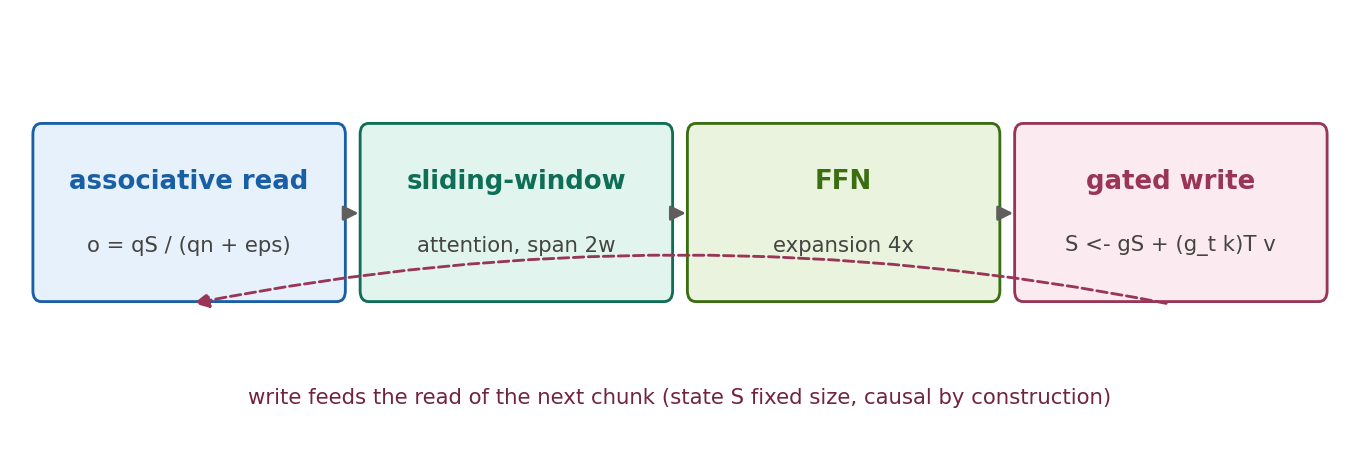
\includegraphics[width=0.95\textwidth]{fig_arch.png}
\caption{One \cmh{} block. Sequences are processed in chunks of $w$ tokens; the dashed
arrow is the cross-chunk recurrence that carries state $S$ (fixed size) from write to
read. Attention inside a chunk is causal over its window; the previous chunk serves as
attend-only context.}
\label{fig:arch}
\end{figure}

\subsection{Engineering notes}

Training uses bf16 autocast, micro-batch gradient accumulation (8 sequences of 512
tokens per micro-step), gradient clipping at 1.0, and AdamW ($\beta_1{=}0.9$,
$\beta_2{=}0.95$, weight decay 0.1). The Python-level chunk loop is unoptimized; a fused
kernel would raise absolute throughput without touching the scaling conclusions.

\section{Why from-scratch training fails}\label{sec:scratch}

\subsection{Diagnostic task}

We probe precise long-range recall with a \emph{copy} task: the input is $L{=}64$ random
tokens (prefix), then a gap of filler tokens, then an echo segment that must re-emit the
prefix. Prediction of echo position $j$ requires retrieving prefix token $j$ over a
distance of $(L + \mathrm{gap})$. With effective window $2w = 256$, gaps beyond
$\sim$192 make the memory channel the only path. Models are causal, trained 3--8k steps
at batch 16, cross-entropy upweighted $8\times$ on echo positions; accuracy is measured
on the 64 echo predictions.

\subsection{Six controlled iterations}

All runs use the same skeleton (8-layer, $d{=}128$ at diagnostic scale) and differ only
in the global channel:

\begin{table}[h]
\centering
\caption{Design iterations on the copy diagnostic. ``gap=32'' is inside the window;
``gap$\ge$192'' requires memory. Full attention reaches $1.00$ and window-only $0.23$
at gap${=}384$ in all rounds.}
\label{tab:iterations}
\begin{tabular}{llll}
\toprule
Iteration & Global channel & gap=32 & gap$\ge$192 \\
\midrule
1 & Softmax memory slots ($M{=}32/64/128$) & 0.03 & $\approx$ random \\
2 & + sigmoid slot gates, sharpened read & 0.03 & $\approx$ random \\
3 & Outer-product associative memory & \textbf{0.69} & 0.03--0.15 \\
4 & + curriculum over gap (32$\to$384) & 0.07 & 0.14 \\
5 & Single head (state $128{\times}128$) & --- & 0.16 (gap 256), 0.25 (gap 320) \\
6 & True sliding window (block-attn bug fixed) & \textbf{0.69} & unchanged \\
\bottomrule
\end{tabular}
\end{table}

\begin{figure}[t]
\centering
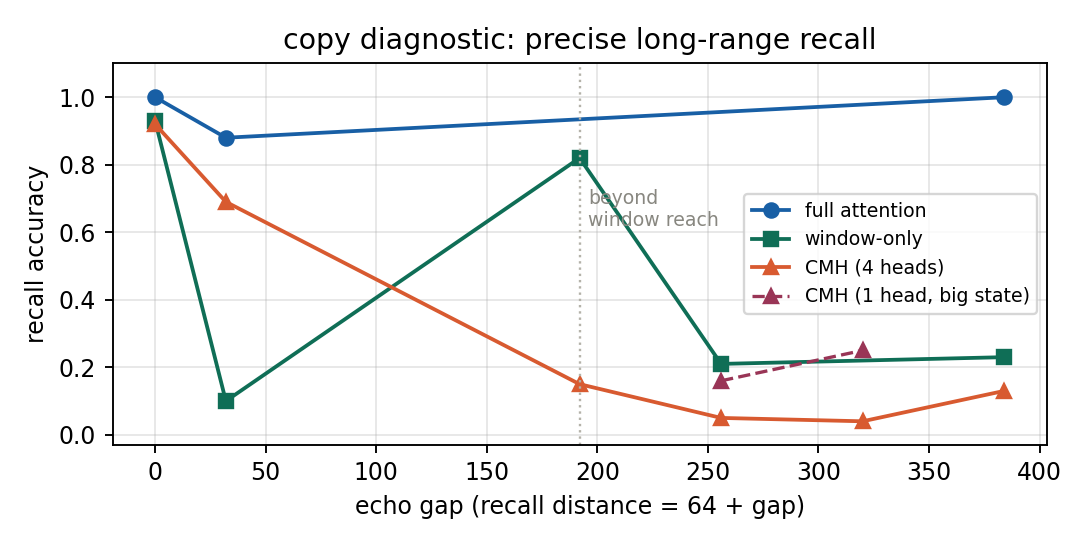
\includegraphics[width=0.95\textwidth]{fig_gapsweep.png}
\caption{Copy-diagnostic recall accuracy against echo gap. The dotted vertical line
marks the point where the prefix falls outside the 256-token effective window; only the
memory channel can bridge it. The single-head variant (dashed) doubles the per-head
state and recovers part of the loss, consistent with the geometric capacity argument in
Section~\ref{sec:derivations}.}
\label{fig:gapsweep}
\end{figure}

Iteration 6 is worth admitting: our first ``window attention'' was in fact non-overlapping
block attention, which left echo tokens blind across chunk boundaries and confounded the
diagnosis of every earlier iteration. Fixing it to a true sliding window changed
within-window results dramatically (window-only baseline at gap${=}$32 from $0.10$ to a
healthy range) but left beyond-window recall unchanged---confirming the memory channel,
not the local channel, is the bottleneck.

\subsection{Root cause: soft-retrieval cold-start}

The read in Eq.~\eqref{eq:read} is a convex combination of stored values weighted by
query--key inner products. For \emph{exact} recall of 64 tokens, the positional
embeddings must first learn a near-orthogonal alignment so that the echo query
$q_{448+j}$ matches prefix key $k_j$ far better than any other key. Before that geometry
exists, the echo query matches all prefix keys roughly equally, and the gradient signal
for sharpening the alignment is spread across all of them---a chicken-and-egg regime we
call \emph{soft-retrieval cold-start}. Softmax attention does not suffer this: its
exponentiation progressively sharpens the strongest match, so full attention bootstraps
the same alignment within $\sim$1,500 steps (loss $6.2 \to 0.05$) where \cmh{} remains
flat at the filler-prediction plateau for $8{,}000$ steps.

Curriculum training (growing the gap from 32 to 384) did not help: the local channel
solves each in-window phase, the memory channel receives no gradient, and the final
out-of-window phase is as cold as before. Enlarging the state (single head,
$128{\times}128$ per layer instead of $4{\times}32{\times}32$) improved beyond-window
recall substantially ($0.04 \to 0.25$ at gap 320, loss still descending at step 3{,}000),
identifying \emph{state capacity and retrieval sharpness} as the binding constraints.

\section{Efficiency evaluation}\label{sec:efficiency}

\cmh{}'s selling point is not single-step absolute speed (the prototype contains an
unoptimized Python chunk loop) but the \emph{scaling curve}. Forward+backward
throughput and peak CUDA memory, batch 8:

\begin{table}[h]
\centering
\caption{Throughput (tokens/s) and peak memory vs.\ sequence length. The \cmh{} numbers
include the unoptimized chunk loop; a fused kernel would improve absolute throughput.}
\label{tab:efficiency}
\begin{tabular}{rrrrr}
\toprule
Seq length & Full-attn tok/s & \cmh{} tok/s & Full-attn peak & \cmh{} peak \\
\midrule
256  & 169{,}730 & 42{,}032 & 0.18 GB & 0.21 GB \\
1024 & 259{,}432 & 40{,}589 & 1.22 GB & 0.87 GB \\
2048 & 146{,}504 & 40{,}502 & 4.29 GB & 1.73 GB \\
4096 & \textbf{2{,}621 (collapse)} & \textbf{39{,}937 (flat)} & \textbf{16.11 GB} & \textbf{3.47 GB} \\
\bottomrule
\end{tabular}
\end{table}

At 4,096 tokens, \cmh{} delivers $15.2\times$ the throughput of full attention with
$78\%$ less peak memory, and both metrics are independent of length. Full attention
collapses as the $O(N^2)$ term dominates.

\begin{figure}[t]
\centering
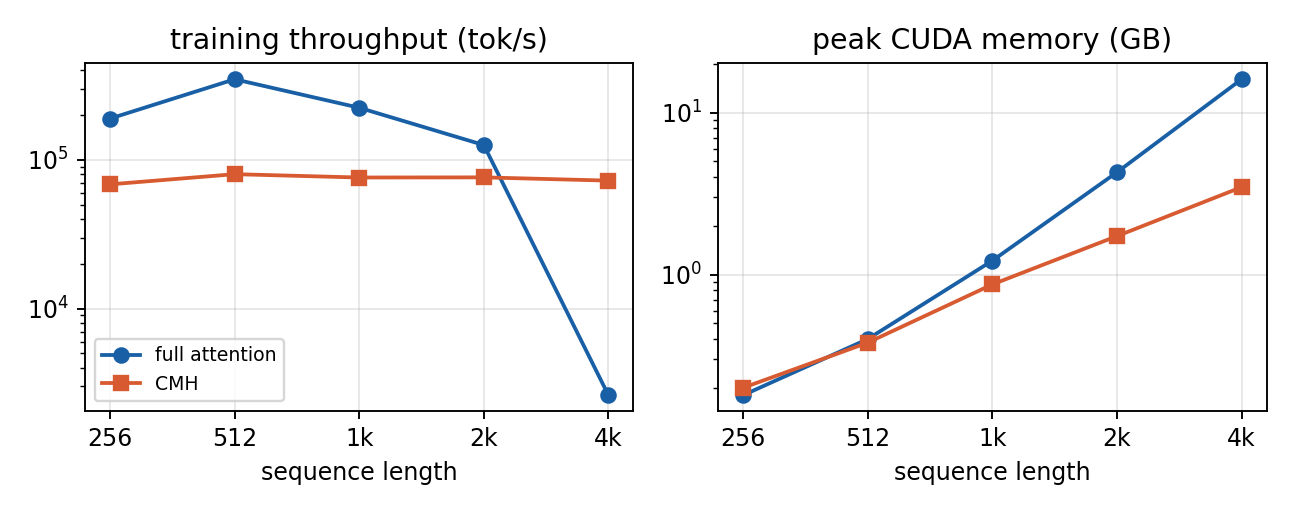
\includegraphics[width=0.95\textwidth]{fig_efficiency.png}
\caption{Throughput (left) and peak CUDA memory (right) against sequence length,
log--log axes. Full attention bends upward in cost and collapses at 4{,}096 tokens;
\cmh{} stays flat.}
\label{fig:efficiency}
\end{figure}

\section{Distillation as the repair path}\label{sec:exp}

\subsection{Setup}

\begin{table}[h]
\centering
\caption{Training configuration.}
\label{tab:setup}
\begin{tabular}{ll}
\toprule
Teacher & GPT-2 (124M), frozen, bf16 forward \\
Students & \cmh{} 38.4M / full 33.7M / window 33.7M (8 layers, $d{=}384$, $h{=}4$, $w{=}256$) \\
Tokenizer & GPT-2 BPE (50{,}257), embedding--head weight tying \\
Data & TinyStories \cite{eldan2023tinystories}, 99M train / 2M val tokens, seq 512 \\
Objective & $\mathcal{L} = \alpha\,\mathrm{CE}(y, p_s) + (1-\alpha)\,T^2\,\mathrm{KL}(\sigma(z_t/T)\,\|\,\sigma(z_s/T))$ \\
KD hyperparams & $T = 2$, $\alpha = 0.5$ \\
Optimizer & AdamW, OneCycle LR $6{\times}10^{-4}$, 6k steps ($\approx$74M tokens), batch 24 \\
\bottomrule
\end{tabular}
\end{table}

The intuition: distillation converts ``what is worth remembering'' from a discovery
problem into a supervised regression problem. The teacher's logits provide a full
distribution at \emph{every} position, giving the write gates, retention rates, and state
content a dense gradient path that bypasses the cold-start regime identified in
Section~\ref{sec:scratch}.

\subsection{Results}

\begin{table}[h]
\centering
\caption{Main results on TinyStories (74M-token training budget, identical data,
tokenizer, and schedule across students).}
\label{tab:main}
\begin{tabular}{lrr}
\toprule
Model & Val CE & Perplexity \\
\midrule
GPT-2 teacher (124M, out-of-domain) & 2.4806 & 11.95 \\
\midrule
scratch-full (33.7M) & \textbf{1.7974} & \textbf{6.03} \\
scratch-window (33.7M) & \textbf{1.7945} & \textbf{6.02} \\
scratch-\cmh{} (38.4M) & 5.4435 & 231.25 \\
\midrule
distill-\cmh{} $\leftarrow$ GPT-2 (38.4M) & 5.4010 & 221.63 \\
distill-\cmh{} $\leftarrow$ full teacher (38.4M) & 5.5556 & 258.69 \\
\bottomrule
\end{tabular}
\end{table}

\begin{figure}[h]
\centering
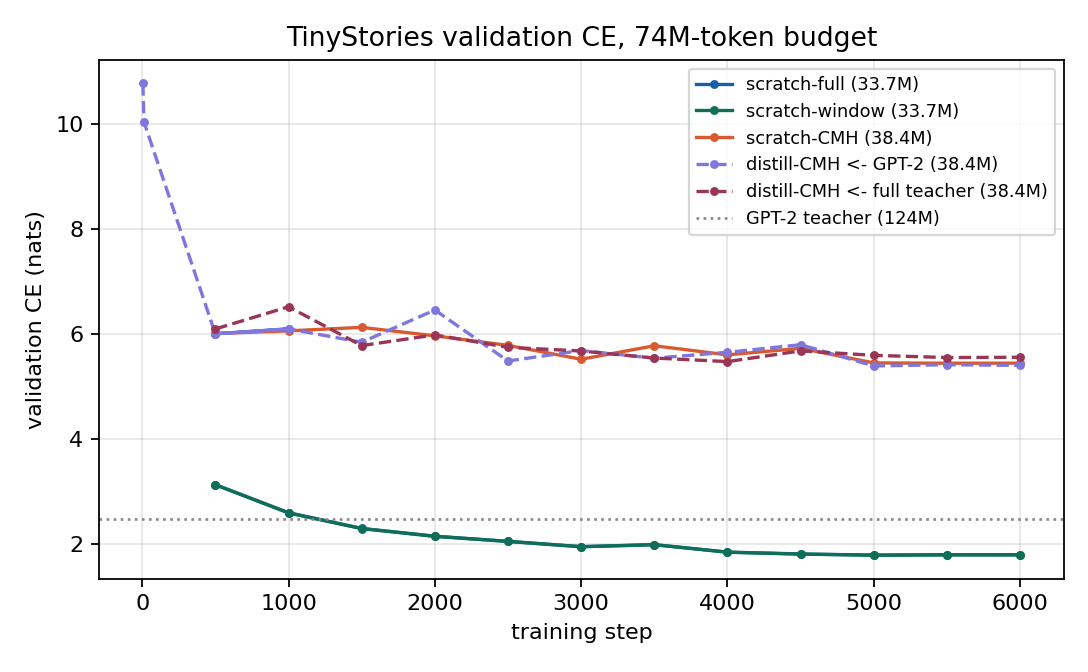
\includegraphics[width=0.85\textwidth]{val_curves.png}
\caption{Validation cross-entropy over training. Dashed lines are distilled students;
the dotted line is the out-of-domain GPT-2 teacher. Window-only matches full attention;
both \cmh{} distillation variants track the from-scratch \cmh{} plateau.}
\label{fig:curves}
\end{figure}

Three observations, all consistent across the full training run:

\textbf{(1) The corpus needs almost no global context.} Window-only matches full
attention to within $0.003$ nats ($1.7945$ vs.\ $1.7974$) at sequence length 512.
Anything a full-attention model can extract beyond a 256-token span, this dataset does
not require---so TinyStories cannot, by itself, demonstrate a value proposition for any
global channel, memory-based or otherwise.

\textbf{(2) The memory channel actively harms.} \cmh{} scores $5.44$ against its own
window-only ablation's $1.79$: the gated associative read (Eq.~\ref{eq:read}) injects a
residual that costs $3.65$ nats rather than contributing information. With more
parameters (38.4M vs.\ 33.7M) the student should dominate in capacity; instead the
soft-associative state is a net liability at this scale.

\textbf{(3) The memory channel is not dead weight --- it is a crutch.} Disabling the
associative read and write at inference (window and FFN unchanged) raises the \cmh{}
student's validation CE from $5.41$ to $6.06$: the state carries about $0.65$ nats of
real signal, and the block has learned to lean on it. But the crutch is what keeps the
model $3.6$ nats behind the window-only model, which needs no crutch at all. We also
inspect the learned retention rates: every head in every layer settles at
$\gamma = 0.924$, barely moved from the $0.951$ initialization, with no head-to-head
specialization --- the ``some heads remember longer'' mechanism we designed for never
engages under the training signal available.

\textbf{(4) Distillation cannot close the gap---from weak or strong teachers.} KD from
GPT-2 yields $-0.04$ nats; KD from an in-domain teacher ($2.48$, itself $0.7$ nats better
than GPT-2 here) yields $+0.11$. Decisively, both distilled students remain
$2.9$--$3.1$ nats \emph{worse than their own teachers}: the student cannot fit the
supervised target distribution itself, so the bottleneck is representational
(the fixed-state read), not the supervision signal. The cold-start hypothesis of
Section~\ref{sec:scratch} is thereby strengthened and made precise: dense per-position
supervision is \emph{necessary but not sufficient}; the architecture must be able to
represent the teacher's addressing behavior for distillation to transfer it.

\section{Discussion and limitations}\label{sec:discussion}

\textbf{What the negative result establishes.} The cold-start analysis is
architecture-specific evidence for a folk theorem, now with a precise boundary: fixed
soft-associative states cannot acquire precise retrieval from sparse task signals
\emph{nor from dense teacher supervision}. The distillation prediction was tested
directly and failed---which shifts responsibility from the training signal to the
representational capacity of the normalized outer-product read.

\textbf{Limitations.} (i) All experiments are at $\le$40M parameters; the scaling
behavior of both the failure and the repair is unverified. (ii) The evaluation corpus is
English children's stories; retrieval-heavy benchmarks (Long Range Arena,
needle-in-a-haystack) are future work. (iii) The student's global channel shares the
read/write parameters across positions; position-specific addressing relies entirely on
learned positional embeddings, which do not extrapolate beyond the training length.
(iv) The memory read is a soft convex combination; hard retrieval (discrete addressing)
is an open alternative.

\textbf{Future work.} (1) Delta-rule writes \cite{yang2023delta}, which allow a written
key to overwrite its own binding and are known to sharpen retrieval. (2) Mixed regimes:
distillation plus a minority of full-attention layers, matching industrial practice.
(3) Scaling studies of whether the memory channel's advantage emerges at larger scale.

\section{Conclusion}

\cmh{} shows that the ``fixed state for $O(N^2)$'' trade pays off exactly on the
efficiency axis: flat throughput to 4{,}096 tokens, $15.2\times$ full attention at
4{,}096, and $78\%$ memory savings. On the quality axis it fails decisively: the gated
associative-memory channel costs $3.65$ nats relative to its own window-only ablation on
real language, and neither from-scratch training nor token-level distillation---from
weak or strong teachers---closes any part of the gap. At sequence lengths where the
corpus needs little global context, sliding-window attention alone matches full
attention; where more is needed, our evidence indicates fixed soft-associative states
cannot provide it at small scale. Hybrid designs that keep explicit full-attention
layers are therefore empirically justified, and progress on this axis likely requires
architecturally different global channels (delta-rule writes, hard addressing, or
learned slot keys) rather than better training signals.

\section*{Acknowledgments}

Code, experiment execution, and drafting were developed with AI coding assistance. All
experimental results were produced by the released scripts and verified against the
training logs; the author reviewed every citation, figure, and claim, and takes full
responsibility for the content. Code, training logs, and the story-continuation demo:
\url{https://github.com/mierstan/CMH}.

\bibliographystyle{plain}
\begin{thebibliography}{20}

\bibitem{vaswani2017} A.~Vaswani et al.
\newblock Attention is all you need.
\newblock \emph{NeurIPS}, 2017.

\bibitem{katharopoulos2020} A.~Katharopoulos, A.~Vyas, N.~Pappas, F.~Fleuret.
\newblock Transformers are RNNs: Fast autoregressive transformers with linear attention.
\newblock \emph{ICML}, 2020.

\bibitem{gu2023mamba} A.~Gu, T.~Dao.
\newblock Mamba: Linear-time sequence modeling with selective state spaces.
\newblock \emph{arXiv:2312.00752}, 2023.

\bibitem{peng2023rwkv} B.~Peng et al.
\newblock RWKV: Reinventing RNNs for the transformer era.
\newblock \emph{EMNLP}, 2023.

\bibitem{yang2023gla} S.~Yang, B.~Wang, Y.~Zhang, Y.~Shen, D.~Schuurmans.
\newblock Gated linear attention transformers with hardware-efficient training.
\newblock \emph{arXiv:2312.06635}, 2023.

\bibitem{sun2023retnet} Y.~Sun et al.
\newblock Retentive network: A successor of transformer for large language models.
\newblock \emph{arXiv:2307.08621}, 2023.

\bibitem{yang2023delta} S.~Yang et al.
\newblock Parallelizing linear transformers with the delta rule over sequence length.
\newblock \emph{arXiv:2406.06484}, 2024.

\bibitem{beltagy2020longformer} I.~Beltagy, M.~E.~Peters, A.~Cohan.
\newblock Longformer: The long-document transformer.
\newblock \emph{arXiv:2004.05168}, 2020.

\bibitem{waleffe2024jamba} R.~Waleffe et al.
\newblock Jamba: A hybrid transformer-Mamba language model.
\newblock \emph{arXiv:2403.19887}, 2024.

\bibitem{glorioso2024zamba} P.~Glorioso et al.
\newblock Zamba: A compact 7B state-space hybrid model.
\newblock \emph{arXiv:2405.16712}, 2024.

\bibitem{wang2024samba} J.~Wang et al.
\newblock Samba: Simple hybrid state space models for efficient unlimited context language modeling.
\newblock \emph{arXiv:2406.07522}, 2024.

\bibitem{wang2024hymba} X.~Wang et al.
\newblock Hymba: A hybrid-head architecture for small language models.
\newblock \emph{arXiv:2411.13676}, 2024.

\bibitem{wang2024mohawk} Y.~Wang et al.
\newblock MOHAWK: Mamba distilled in the trenches of long context.
\newblock \emph{arXiv:2408.00140}, 2024.

\bibitem{wang2024mambaillama} J.~Wang et al.
\newblock Mamba in the Llama: Distilling and accelerating hybrid models.
\newblock \emph{arXiv:2408.04029}, 2024.

\bibitem{hinton2015distill} G.~Hinton, O.~Vinyals, J.~Dean.
\newblock Distilling the knowledge in a neural network.
\newblock \emph{arXiv:1503.02531}, 2015.

\bibitem{eldan2023tinystories} R.~Eldan, Y.~Li.
\newblock TinyStories: How small can language models be and still speak coherent English?
\newblock \emph{arXiv:2305.07759}, 2023.

\end{thebibliography}

\end{document}
